\documentclass{standalone}
\usepackage{pgfplots}
\pgfplotsset{compat = newest}

\begin{document}
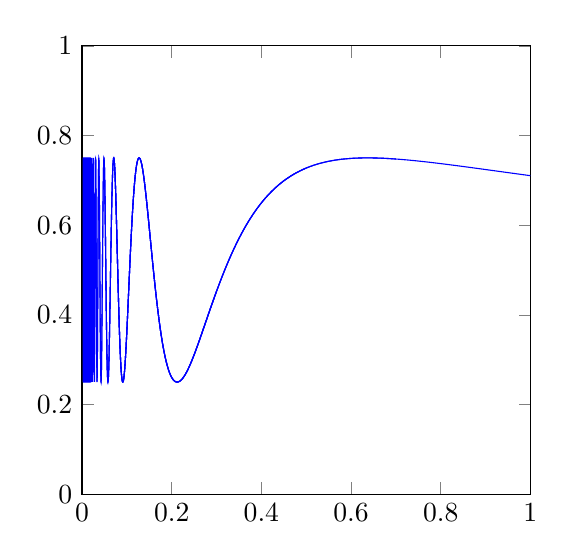
\begin{tikzpicture}
    \begin{axis}[xmin=0,xmax=1,ymin=0,ymax=1,
        axis equal image]
        \addplot [thin,samples=200,smooth,blue,domain=0.2:1] {0.25 * sin(deg(1/x))+0.5};
        \addplot [thin,samples=2000,smooth,blue,domain=0.1:0.2] {0.25 * sin(deg(1/x))+0.5};
        \addplot [thin,samples=1000,smooth,blue,domain=0.07:0.1] {0.25 * sin(deg(1/x))+0.5};
        \addplot [thin,samples=1000,smooth,blue,domain=0.05:0.7] {0.25 * sin(deg(1/x))+0.5};
        \addplot [thin,samples=1000,smooth,blue,domain=0.03:0.5] {0.25 * sin(deg(1/x))+0.5};
        \addplot [thin,samples=2000,smooth,blue,domain=0.019:0.3] {0.25 * sin(deg(1/x))+0.5};
        \draw [rounded corners=0.1pt,thin,blue,fill=blue] (0.0025,0.75) rectangle (0.019,0.25);
        \end{axis}
\end{tikzpicture}
\end{document}